% !TEX root = dissertationmain.tex
%Chapter
\chapter{Methodology}
\label{chap:brief}
%Brief
\paragraph{}This chapter contains an in-depth analysis of the design and implementation stages carried out during this project. Initially, the design and goals of the application will be enumerated. Subsequently an analysis of the application’s infrastructure will be presented followed by an in-depth detail of the modules and submodules within the application’s programming. A test case scenario will be defined and executed to provide a proof of concept. The efficiency and accuracy among other factors based on the test scenario will be analysed during the discussion chapter of this thesis. 

%Section
\section{Design}
\label{sec:design}

\paragraph{}The application design’s primary goal was to be able to detect vulnerable machines on a large-scale network infrastructure regardless of topology or host types by using machine learning techniques and automated tool outputs. However, there are several requirements the application must adhere to for it to be a viable tool during a security assessment. The application created for this thesis was done so strictly on a proof of concept bases.\linebreak

The application was designed with the following requirements in mind:

\paragraph{}\textbf{Text progress output with multiple verbosity settings} allowing for an experienced tester to understand what the application is doing at any point in time during execution. This is critical as tools used during an assessment on live networks must not hinder or damage the network or its hosts in any way as to disrupt an organisations business.

\paragraph{}\textbf{Several input type parameters} for which the tester can utilise based on the current information known about the network. Such as only using one type of scan file and manually selecting the clustering model. 

\paragraph{}\textbf{Several output options including visually in the form of graphs} and to a dot type file to be used with other industry applications and reports.

\paragraph{}\textbf{Manual overriding of variables via parameters} in order to allow for the application to be scripted and modified by the tester. This will increase the efficiency of using the tool and provide advanced customisation of the algorithms within the application.

\paragraph{}\textbf{Highly versatile with working conditions and configurability.} The programming of the application to be highly documented allowing a tester to fix and modify the application code to suit the operation’s needs. By using a primarily interpreted language as appose to compiled one would allow for this, as well as making the application portable without extra code. For these purposes, the Python programming language was chosen. With the majority of modern tools and scripts used by penetration testers haven been written in Python due to its versatility, reliability and portability, it further enforces this choice.


\subsection{Application Brief}

\paragraph{}The application requires several parameters to run and has three different global modes; manual, assisted and automatic. These modes can either be run with Nmap, Nessus or both inputs with the majority of the use case scenarios requiring both. The application will then parse these inputs, process the data in several ways and cluster the information based on feature similarities. Output includes the full details of each cluster within the clustering. If using both inputs the application will combine the data from each and subtract large similarity clusters. By doing this, the application will determine the most unique hosts within the topology and display them in a new clustering. The unique hosts will, based on probability, be the most vulnerable on the network and should be prioritised by a tester during the manual assessment. This is due to the model prioritising the vulnerabilities each scanner detects then appends them to the pre-existing host set, thus rendering that host more unique than the others.

\paragraph{}An example output of the application when using \textbf{twin input automatic mode} can be found in text form using maximum verbose level at Appendix \ref{exampleoutput} and a Figure of the graphing interface GUI at Appendix \ref{example_twin}. The data-set used for these examples were Nessus and Nmap scan XML outputs generated from a fictional network. Due to the sensitive nature of the data included within these scans such as SSH keys and vulnerability codes, there are no publicly available data-sets.\linebreak

The difference between modes and parameters will be explained within the next section \textit{infrastructure analyses.}

%Section
\section{Infrastructure}
\label{sec:infrastructure}

\begin{figure}[!h]
\centering
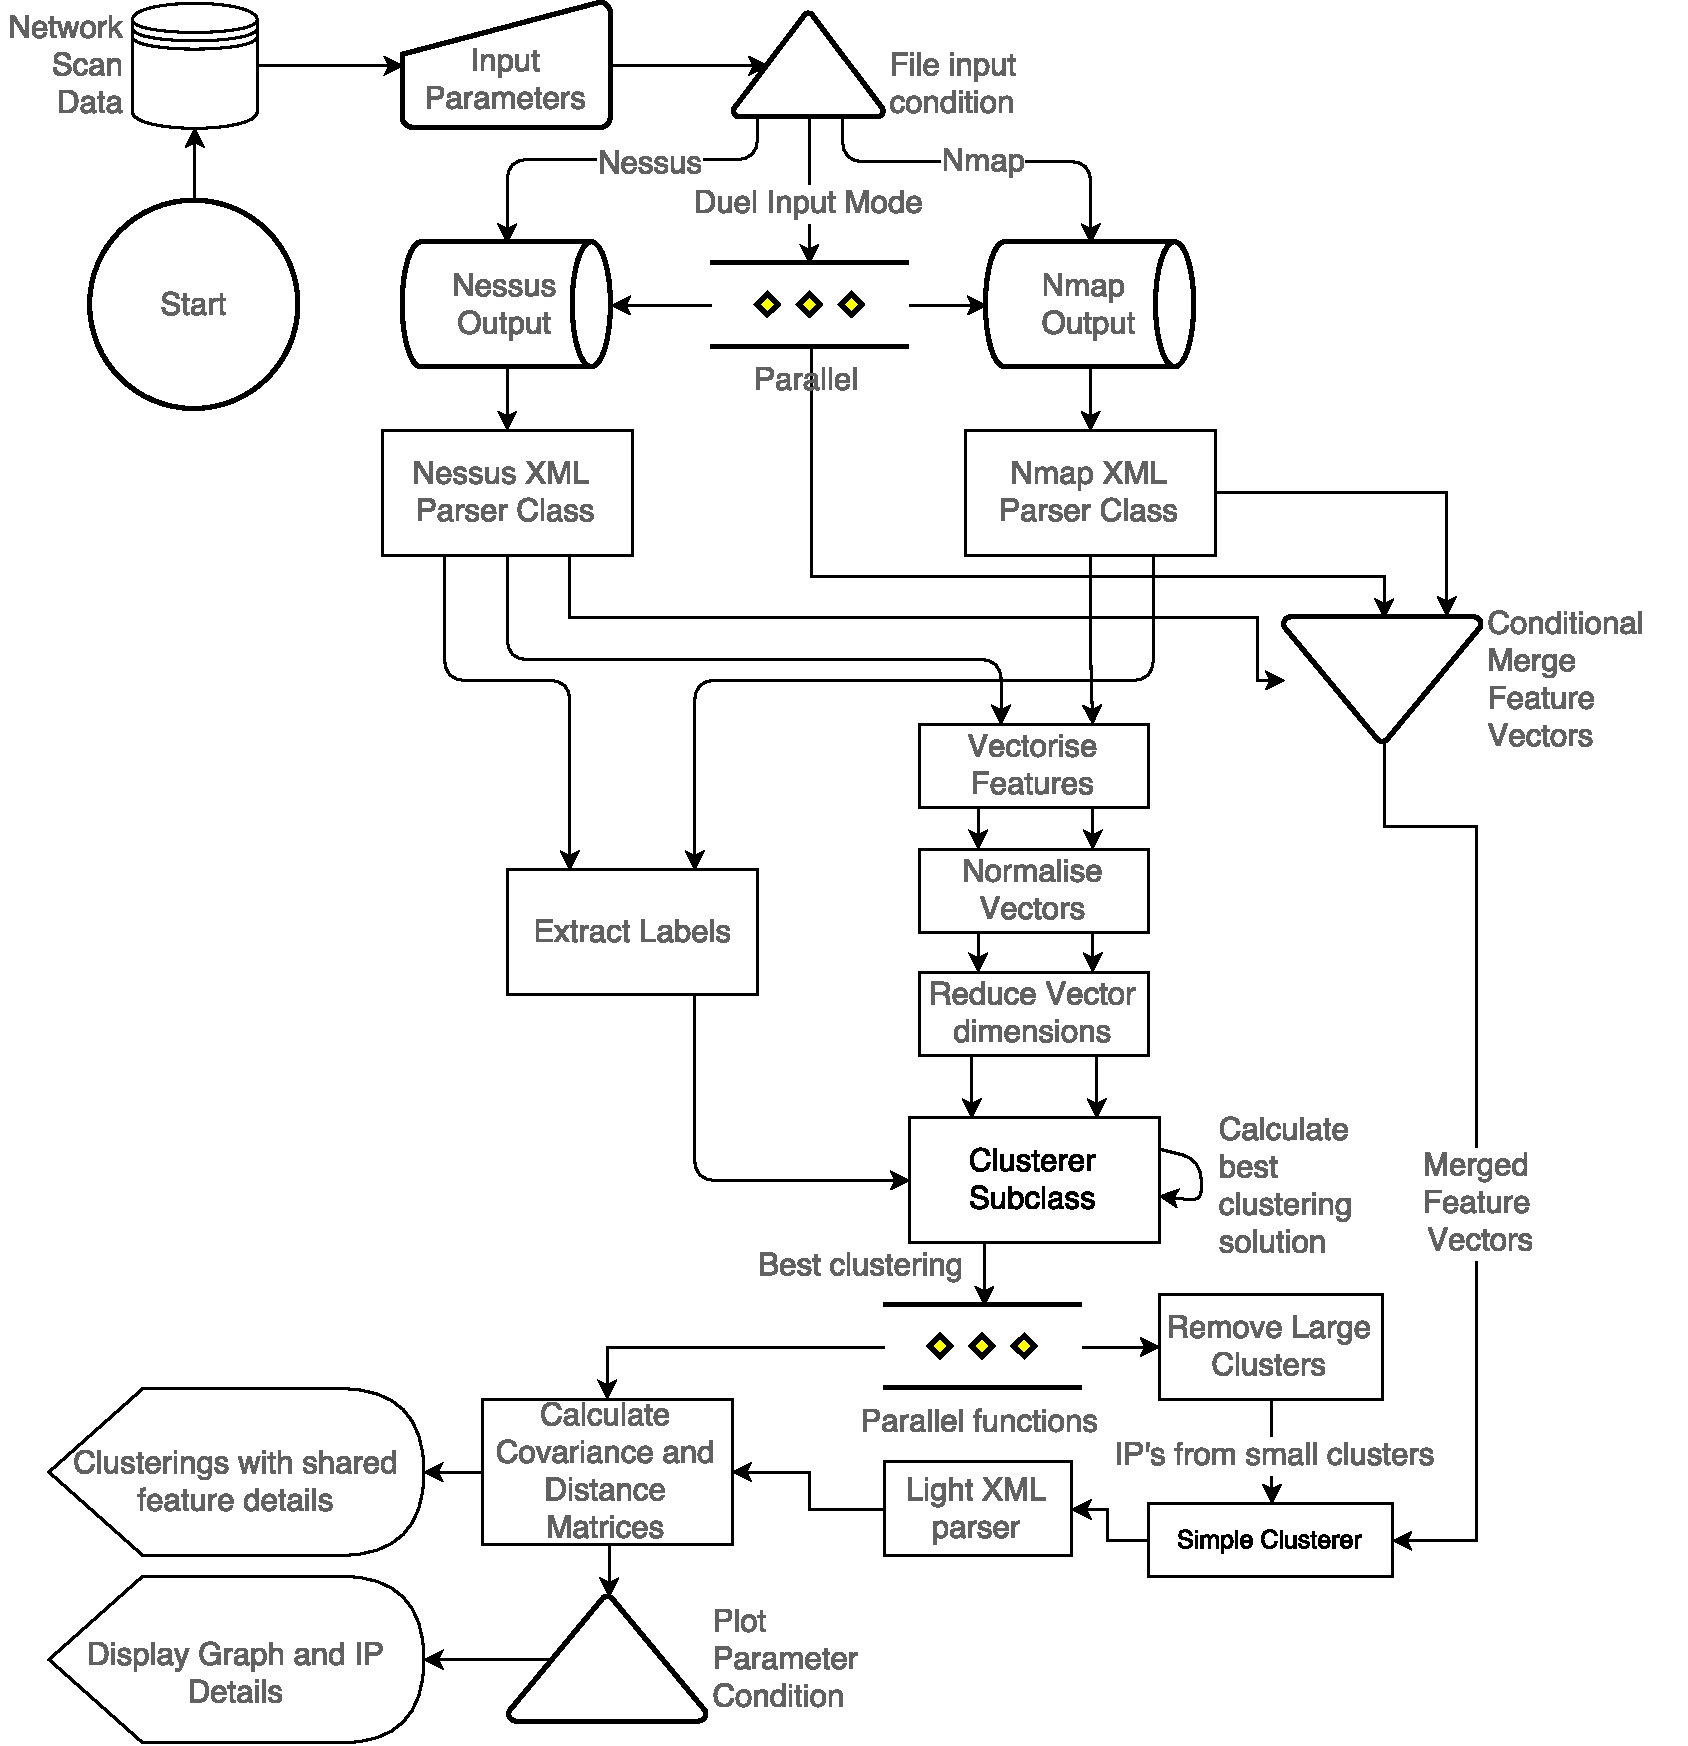
\includegraphics[width=4.5in]{./Figures/flow.pdf}
\caption{Application infrastructure data flow diagram}
\label{flow}
\end{figure}

\paragraph{}Figure \ref{flow} shows the application’s primary class infrastructure when in automatic mode. The infrastructure diagram has been created using standard flow diagram symbols to provide understanding of the process types. The application has been programmed for python version 2.7 interpreters and therefore will not have complete functionality without modification for python 3.0 and above. Due to time constraints placed upon this thesis the library NMAP-Cluster, \cite{blackhatnmap}, was used to conserve time.

\paragraph{}In order to execute this application, it is important to have the correct library dependences. This is done via the python package manager ‘PIP’ and a requirements file, found in Appendix \ref{requirementsfile}, by executing the command:
\lstset{language=Python}
\begin{lstlisting}
Pip install -r requirements.txt
\end{lstlisting}

\paragraph{}The following sections include detailed descriptions of the processes symbolised within the infrastructure Figure \ref{flow}.  Beginning from the start circle and ending at the display modules.\linebreak

\subsection{Usage and Parameters}
\label{infra1}

\begin{figure}[!h]
\centering
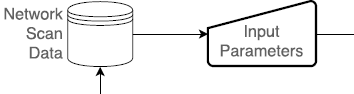
\includegraphics{./Figures/infra1.png}
\caption{Network scan data and input parameter modules from infrastructure diagram at Figure \ref{flow}}
\label{infra1}
\end{figure}
The modules shown in Figure \ref{infra1} are those used to store the network scan data and process the applications input parameters. The Network Scan Data module refers to the XML output of an Nmap scan, Nessus proprietary export file or both. These must be in their respectable formats in order for the parser to recognise them. The files must also be referenced in their correct positional arguments when executing the application such as mentioned in the application usage in Appendix \ref{usage}.

\paragraph{}The  manual input parameters module on Figure \ref{infra1} refers to the parameters that the application requires to select the correct run configuration. This is required because the application has no execution graphical user interface (GUI), the lack of which was decided for several reasons. Such as allowing for scripting, verbose output and terminal pipe operation commands. This type of interface is generally preferred by professionals due to the speed and reliability it provides over a standard GUI. The graphing stage of the application does however, provide a GUI to allow for manipulation of the graphs in multiple ways. The application usage found in Appendix \ref{usage} includes a full description of the possible parameters. The parameters are passed into the data processing section of the application explained in the next session. The three possible run modes are explained in a later section \ref{modes}.

\subsection{Data Processing}
\label{infra2}

\begin{figure}[!h]
\centering
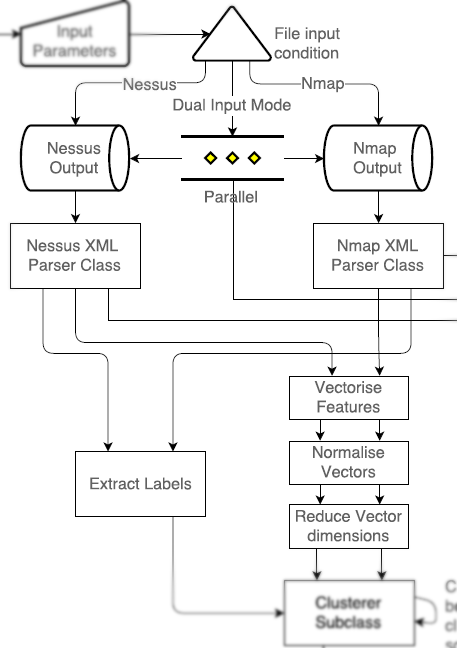
\includegraphics[width=3.5in]{./Figures/infra2.png}
\caption{The data processing section from the infrastructure diagram at Figure \ref{flow} with the irrelevant modules blurred out}
\label{infra2}
\end{figure}

Figure \ref{infra2} displays the data processing section of the application, an analysis of this section is provided in the following paragraphs. \paragraph{}Depending on the files specified within  the input parameters, the application will either feed the Nessus, Nmap or both XML files into the parser classes. These parser classes will take the data from each file and transform it into IP addresses and features which are then passed individually into vectorizers. Vectorization is required for the features to be understood by the clustering algorithm. Vectorization refers to the general process of turning a collection of text (in this case machine attributes) into numerical feature vectors. It is important to note that data from each scanner file is kept separate until the final process. The vectorization class is short and concise due to it having only two purposes, to call the parsers and vectorise the returned results. More information on the vectorization of each file as well as the raw python class code can be found in Appendix \ref{vectorize.py}.

\paragraph{}Once the data has been vectorised it must be normalised in order to avoid large value bias when using dimensionality reduction algorithms such as PCA. Data normalization scales the values to within the same range whilst keeping the data variance and eliminating the bias problem. This is programmed immediately after vectorisation in the applications initialisation class found in its raw code form at Appendix \ref{cluster.py}.

\paragraph{}The major difference between each scanner used is that the Nessus output values include vulnerabilities over Nmap which has superior information on the services and ports of the machine. By using both, the optimal range of information can be achieved, however, this introduces the problem of overfitting which PCA has countered. For more information on PCA refer to dimensionality reduction section \ref{pca} in the introduction. It is possible to greatly modify the output of the two scanners by either using scripts with Nmap or custom plugins for Nessus. Due to the modularity of the application, these modifications to the scanners will not affect the parsers and therefore can be used safely. PCA is also implemented within the initialisation class which can be found in Appendix \ref{cluster.py}. Once PCA is complete, the still separated feature vectors are sent to the clusterer subclass and possibly the conditional merger. The following section will explain the conditional merger of which is represented by symbol in Figure \ref{CMFV}.

\subsection{Small Combined Cluster}
\label{infra3}

\begin{figure}[!h]
\centering
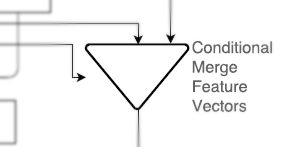
\includegraphics{./Figures/CMFV.png}
\caption{Conditional merge vectors process module from the infrastructure diagram at Figure \ref{flow}}
\label{CMFV}
\end{figure}

\paragraph{}The conditional process of merging the feature vectors, referred to by the symbol in Figure \ref{CMFV}, is executed at this stage, condition dependant on whether dual input mode has been selected when initialising the applications parameters. However, this path must then pause until the main cluster subclass (as represented by the symbol in Figure \ref{clustersub}.) has completed in order to use its clustering outputs. Once this has occurred, each clustering will be duplicated and the large clusters with greater than three IP addresses will be removed from the clustering. This value can be changed based on the network size however the value of three was found to be optimal for networks of size 10 to 1000 from the algorithm tuning stage. The result of each is combined then re-clustered and the remaining IP’s passed through a simpler file parser (compared to that of the ones previously used) to retrieve the information in an un-vectorised text format. This is done to display individual machine information for the end user within the graphing interface. The main cluster subclass mentioned previously is explained in the following section.

\subsection{Clustering Algorithm}
\label{infra4}

\begin{figure}[!h]
\centering
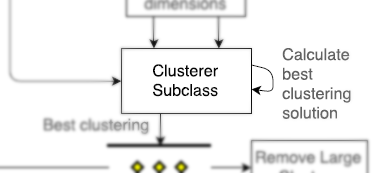
\includegraphics{./Figures/clustersubclass.png}
\caption{Representation of clusterer subclass from infrastructure diagram Figure \ref{flow} spotlighted}
\label{clustersub}
\end{figure}

\paragraph{}The Clusterer subclass represented in the infrastructure diagram by the symbol in Figure \ref{clustersub} above is where the majority of the calculations are done within the application. This includes the three different modes; manual, assisted and automatic. The raw python code for this module can be found in Appendix \ref{cluster_subclass}. *INCOMPLETE*

\subsection{Covariance and Distance Matrices}
\label{infra5}

\begin{figure}[!h]
\centering
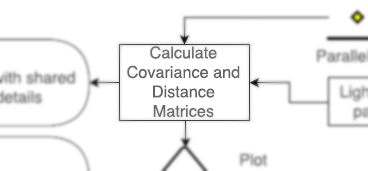
\includegraphics{./Figures/cov.png}
\caption{Representation of covariance and distance matrices function from infrastructure diagram Figure \ref{flow} spotlighted}
\label{cov}
\end{figure}

\paragraph{}Covariance and distance matrices are calculated just before displaying the graphing interface. The function symbol is shown in Figure \ref{cov} above. The output from these functions can be found at the end of the text output, an example is shown in Appendix \ref{exampleoutput}. This is shown for the simple purpose of giving a technical user the knowledge of the used data-set. Specifically, the covariance matrix shows how related the centroids for each clustering are to each other. Whilst the Distance matrix shows the distance between each clustering centroid. These calculations are done for each clustering in the current mode (e.g. three times if using twin mode) however, they only shown in verbose level one and above.

\subsection{Display Modules}
\label{infra6}

\begin{figure}[!h]
\centering
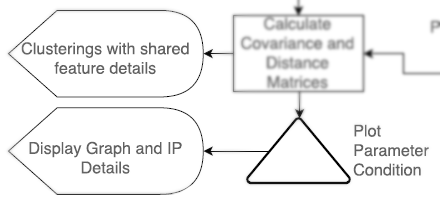
\includegraphics{./Figures/display.png}
\caption{Representation of the display modules from infrastructure diagram Figure \ref{flow} with irrelevant modules blurred out}
\label{display}
\end{figure}


The application will display the main output at the end of its execution as shown in the infrastructure diagram with the symbol from Figure \ref{display}. The application will show a running output as the calculations are performed providing that the verbosity level is set to one or higher. The verbosity parameter will only effect the text output and not the graphing interface of the application. Without verbose output selected the text output will only show the cluster details (for both formats if using twin mode)  *INCOMPLETE*

Modes and parameters. Usage examples.


\newpage
TODO notes
\begin{itemize}
\item complete cluster sub class description and display description such as Gap statistic- http://web.stanford.edu/~hastie/Papers/gap.pdf and The elbow method
\item Modes and parameters. Usage examples. - describe them in depth
\item mathematical model
\item POC testing, what was done. Validate results
\end{itemize}



%Section
\section{Proof of Concept Testing}
\label{poc}


